\documentclass{standalone}
\usepackage{tikz}
\usetikzlibrary{patterns, positioning}
\usepackage[sfdefault]{ClearSans} %% option 'sfdefault' activates Clear Sans as the default text font
\usepackage[T1]{fontenc}

\begin{document}
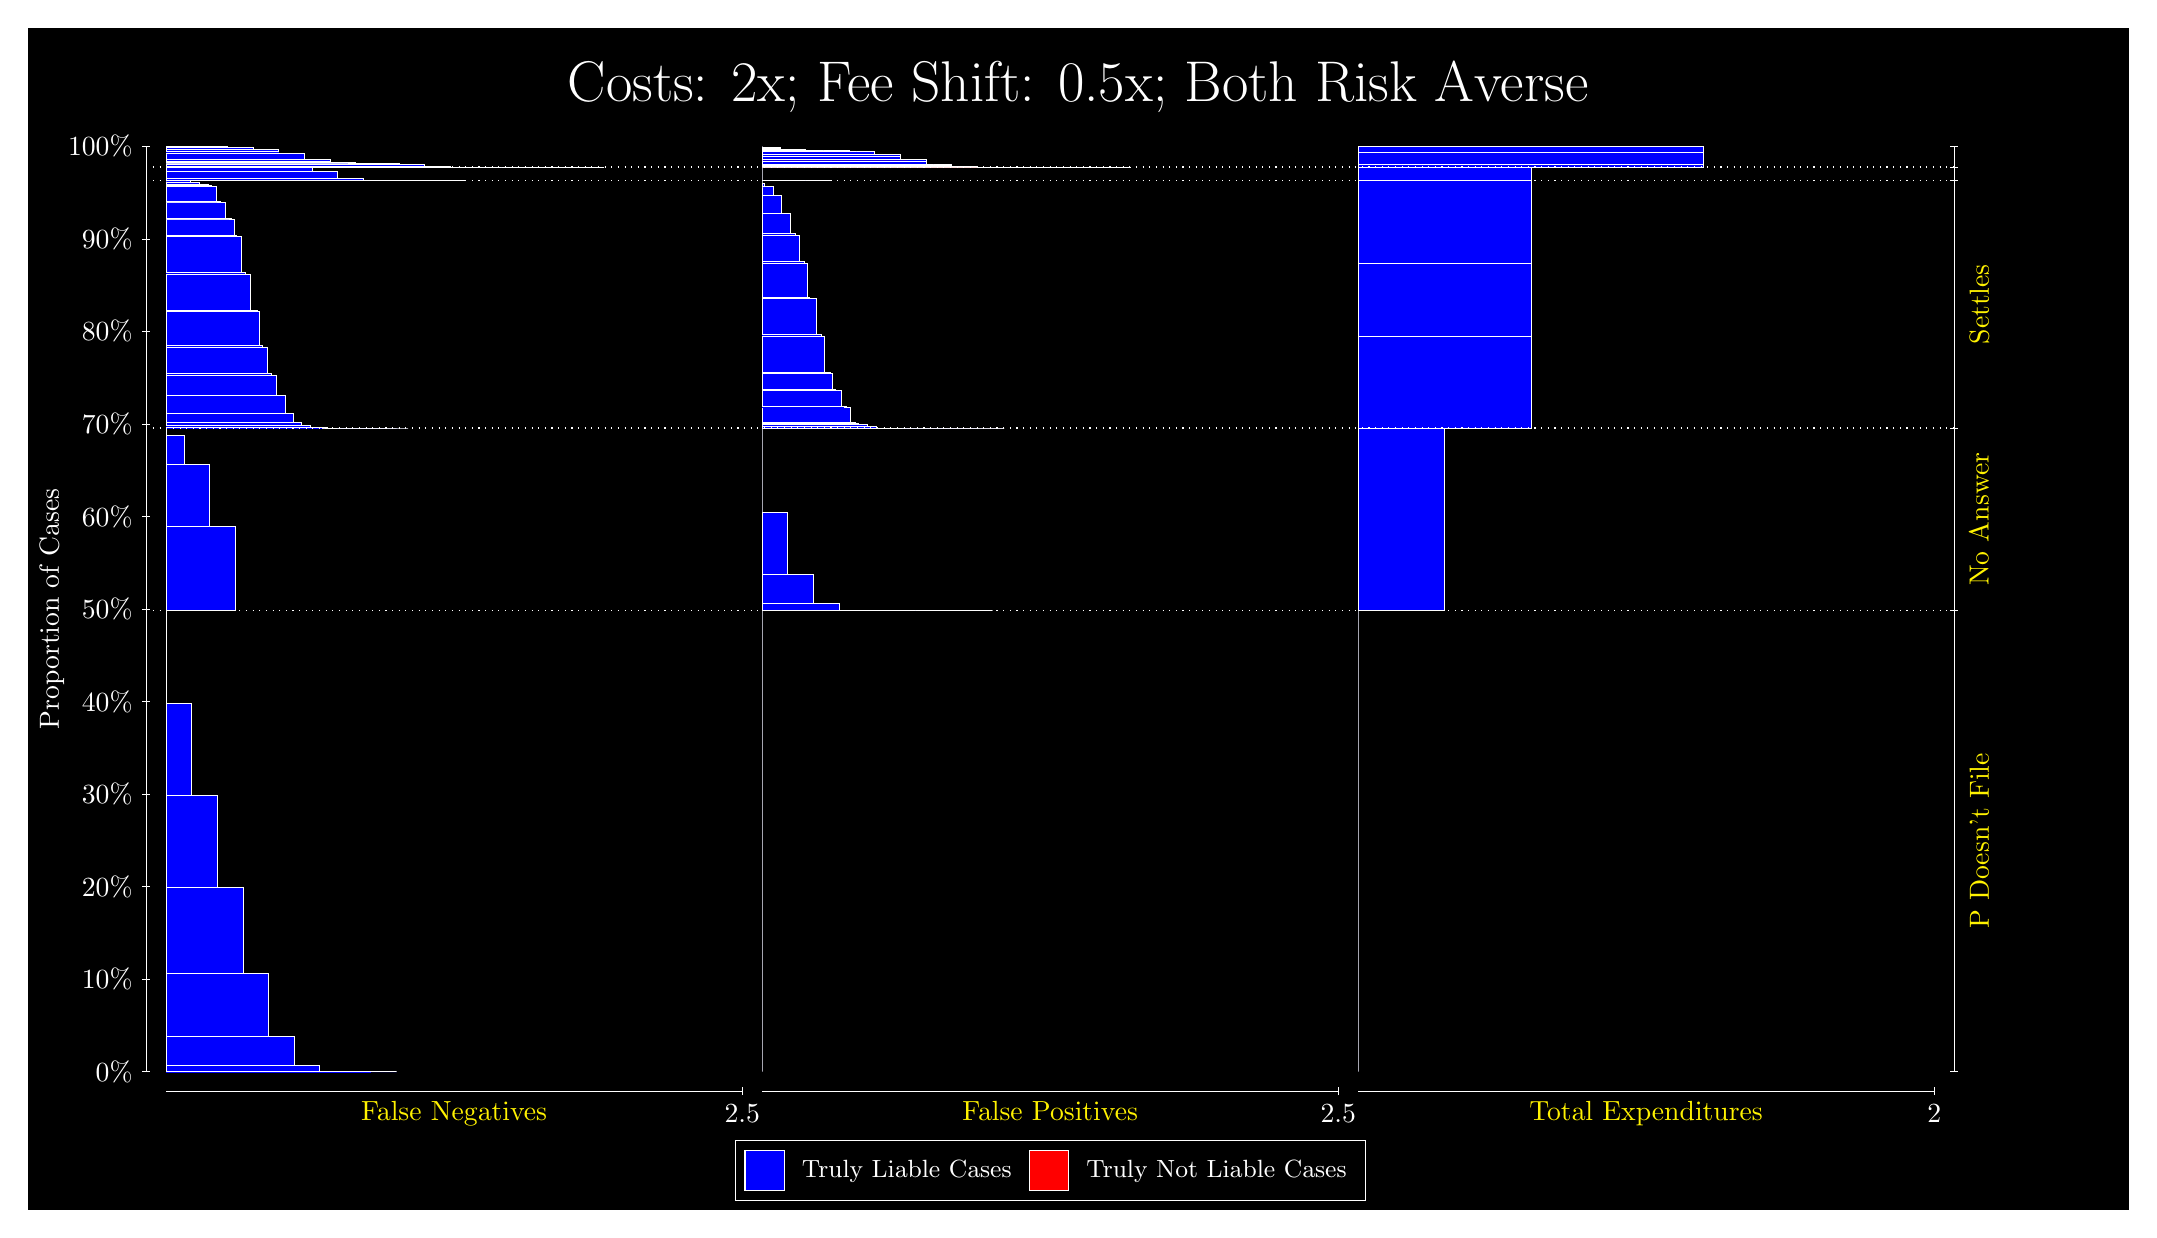
\begin{tikzpicture}
\draw[fill=black] (0,0) rectangle (26.667,15);
\draw[text=white] (0,13.5) rectangle (26.667,15) node[midway] {\huge Costs: 2x; Fee Shift: 0.5x; Both Risk Averse};
\draw[white, very thin] (1.5,1.75) -- (1.5,13.5);
\node[rotate=90, text=white, anchor=center] at (0.3, 7.625) {Proportion of Cases};
\draw[white, very thin] (1.45,1.75) -- (1.55,1.75);
\node[text=white, anchor=east] at (1.45, 1.75) {0\%};
\draw[white, very thin] (1.45,2.925) -- (1.55,2.925);
\node[text=white, anchor=east] at (1.45, 2.925) {10\%};
\draw[white, very thin] (1.45,4.1) -- (1.55,4.1);
\node[text=white, anchor=east] at (1.45, 4.1) {20\%};
\draw[white, very thin] (1.45,5.275) -- (1.55,5.275);
\node[text=white, anchor=east] at (1.45, 5.275) {30\%};
\draw[white, very thin] (1.45,6.45) -- (1.55,6.45);
\node[text=white, anchor=east] at (1.45, 6.45) {40\%};
\draw[white, very thin] (1.45,7.625) -- (1.55,7.625);
\node[text=white, anchor=east] at (1.45, 7.625) {50\%};
\draw[white, very thin] (1.45,8.8) -- (1.55,8.8);
\node[text=white, anchor=east] at (1.45, 8.8) {60\%};
\draw[white, very thin] (1.45,9.975) -- (1.55,9.975);
\node[text=white, anchor=east] at (1.45, 9.975) {70\%};
\draw[white, very thin] (1.45,11.15) -- (1.55,11.15);
\node[text=white, anchor=east] at (1.45, 11.15) {80\%};
\draw[white, very thin] (1.45,12.325) -- (1.55,12.325);
\node[text=white, anchor=east] at (1.45, 12.325) {90\%};
\draw[white, very thin] (1.45,13.5) -- (1.55,13.5);
\node[text=white, anchor=east] at (1.45, 13.5) {100\%};

\draw[white, very thin] (24.457,1.75) -- (24.457,13.5);
\draw[white, very thin] (24.407,1.75) -- (24.507,1.75);
\node[anchor=west] at (24.407, 1.75) {};
\draw[white, very thin] (24.407,7.6064) -- (24.507,7.6064);
\node[anchor=west] at (24.407, 7.6064) {};
\draw[white, very thin] (24.407,9.9227) -- (24.507,9.9227);
\node[anchor=west] at (24.407, 9.9227) {};
\draw[white, very thin] (24.407,13.066) -- (24.507,13.066);
\node[anchor=west] at (24.407, 13.066) {};
\draw[white, very thin] (24.407,13.237) -- (24.507,13.237);
\node[anchor=west] at (24.407, 13.237) {};
\draw[white, very thin] (24.407,13.5) -- (24.507,13.5);
\node[anchor=west] at (24.407, 13.5) {};

\draw[white, very thin, fill=blue] (1.75,1.75) rectangle (4.6775,1.75);
\draw[white, very thin, fill=blue] (1.75,1.75) rectangle (4.3523,1.7503);
\draw[white, very thin, fill=blue] (1.75,1.7503) rectangle (4.027,1.7575);
\draw[white, very thin, fill=blue] (1.75,1.7575) rectangle (3.7017,1.8349);
\draw[white, very thin, fill=blue] (1.75,1.8349) rectangle (3.3764,2.193);
\draw[white, very thin, fill=blue] (1.75,2.193) rectangle (3.0511,2.9983);
\draw[white, very thin, fill=blue] (1.75,2.9983) rectangle (2.7258,4.0903);
\draw[white, very thin, fill=blue] (1.75,4.0903) rectangle (2.4006,5.2569);
\draw[white, very thin, fill=blue] (1.75,5.2569) rectangle (2.0753,6.4315);
\draw[white, very thin, fill=red] (1.75,6.4315) rectangle (1.75,6.4315);
\draw[white, very thin, fill=blue] (1.75,6.4315) rectangle (1.75,7.6064);
\draw[white, very thin, fill=blue] (1.75,7.6064) rectangle (2.6283,8.671);
\draw[white, very thin, fill=blue] (1.75,8.671) rectangle (2.303,9.4664);
\draw[white, very thin, fill=blue] (1.75,9.4664) rectangle (1.9777,9.835);
\draw[white, very thin, fill=red] (1.75,9.835) rectangle (1.75,9.835);
\draw[white, very thin, fill=blue] (1.75,9.835) rectangle (1.75,9.9227);
\draw[white, very thin, fill=blue] (1.75,9.9227) rectangle (4.8239,9.9227);
\draw[white, very thin, fill=blue] (1.75,9.9227) rectangle (4.6775,9.9227);
\draw[white, very thin, fill=blue] (1.75,9.9227) rectangle (4.5312,9.9227);
\draw[white, very thin, fill=blue] (1.75,9.9227) rectangle (4.4986,9.9227);
\draw[white, very thin, fill=blue] (1.75,9.9227) rectangle (4.3848,9.9227);
\draw[white, very thin, fill=blue] (1.75,9.9227) rectangle (4.3523,9.9227);
\draw[white, very thin, fill=blue] (1.75,9.9227) rectangle (4.2384,9.9227);
\draw[white, very thin, fill=blue] (1.75,9.9227) rectangle (4.2059,9.9227);
\draw[white, very thin, fill=blue] (1.75,9.9227) rectangle (4.1734,9.9227);
\draw[white, very thin, fill=blue] (1.75,9.9227) rectangle (4.092,9.9227);
\draw[white, very thin, fill=blue] (1.75,9.9227) rectangle (4.0595,9.9227);
\draw[white, very thin, fill=blue] (1.75,9.9227) rectangle (4.027,9.9227);
\draw[white, very thin, fill=blue] (1.75,9.9227) rectangle (3.9457,9.9227);
\draw[white, very thin, fill=blue] (1.75,9.9227) rectangle (3.9131,9.9235);
\draw[white, very thin, fill=blue] (1.75,9.9235) rectangle (3.8806,9.9235);
\draw[white, very thin, fill=blue] (1.75,9.9235) rectangle (3.8481,9.9235);
\draw[white, very thin, fill=blue] (1.75,9.9235) rectangle (3.7993,9.9257);
\draw[white, very thin, fill=blue] (1.75,9.9257) rectangle (3.7668,9.9257);
\draw[white, very thin, fill=blue] (1.75,9.9257) rectangle (3.7342,9.9261);
\draw[white, very thin, fill=blue] (1.75,9.9261) rectangle (3.7017,9.9262);
\draw[white, very thin, fill=blue] (1.75,9.9262) rectangle (3.6204,9.9264);
\draw[white, very thin, fill=blue] (1.75,9.9264) rectangle (3.5878,9.9538);
\draw[white, very thin, fill=blue] (1.75,9.9538) rectangle (3.5553,9.9542);
\draw[white, very thin, fill=blue] (1.75,9.9542) rectangle (3.5228,9.9543);
\draw[white, very thin, fill=blue] (1.75,9.9543) rectangle (3.474,9.9929);
\draw[white, very thin, fill=blue] (1.75,9.9929) rectangle (3.4415,9.9929);
\draw[white, very thin, fill=blue] (1.75,9.9929) rectangle (3.4089,10);
\draw[white, very thin, fill=blue] (1.75,10) rectangle (3.3764,10.001);
\draw[white, very thin, fill=blue] (1.75,10.001) rectangle (3.3602,10.108);
\draw[white, very thin, fill=blue] (1.75,10.108) rectangle (3.2951,10.112);
\draw[white, very thin, fill=blue] (1.75,10.112) rectangle (3.2626,10.338);
\draw[white, very thin, fill=blue] (1.75,10.338) rectangle (3.23,10.342);
\draw[white, very thin, fill=blue] (1.75,10.342) rectangle (3.1975,10.343);
\draw[white, very thin, fill=blue] (1.75,10.343) rectangle (3.1487,10.595);
\draw[white, very thin, fill=blue] (1.75,10.595) rectangle (3.1162,10.596);
\draw[white, very thin, fill=blue] (1.75,10.596) rectangle (3.0837,10.62);
\draw[white, very thin, fill=blue] (1.75,10.62) rectangle (3.0511,10.621);
\draw[white, very thin, fill=blue] (1.75,10.621) rectangle (3.0349,10.954);
\draw[white, very thin, fill=blue] (1.75,10.954) rectangle (2.9698,10.969);
\draw[white, very thin, fill=blue] (1.75,10.969) rectangle (2.9373,11.409);
\draw[white, very thin, fill=blue] (1.75,11.409) rectangle (2.9048,11.417);
\draw[white, very thin, fill=blue] (1.75,11.417) rectangle (2.8722,11.418);
\draw[white, very thin, fill=blue] (1.75,11.418) rectangle (2.8234,11.879);
\draw[white, very thin, fill=blue] (1.75,11.879) rectangle (2.7909,11.88);
\draw[white, very thin, fill=blue] (1.75,11.88) rectangle (2.7584,11.895);
\draw[white, very thin, fill=blue] (1.75,11.895) rectangle (2.7258,11.896);
\draw[white, very thin, fill=blue] (1.75,11.896) rectangle (2.7096,12.361);
\draw[white, very thin, fill=blue] (1.75,12.361) rectangle (2.6445,12.372);
\draw[white, very thin, fill=blue] (1.75,12.372) rectangle (2.612,12.579);
\draw[white, very thin, fill=blue] (1.75,12.579) rectangle (2.5795,12.582);
\draw[white, very thin, fill=blue] (1.75,12.582) rectangle (2.5469,12.582);
\draw[white, very thin, fill=blue] (1.75,12.582) rectangle (2.4982,12.794);
\draw[white, very thin, fill=blue] (1.75,12.794) rectangle (2.4656,12.794);
\draw[white, very thin, fill=blue] (1.75,12.794) rectangle (2.4331,12.796);
\draw[white, very thin, fill=blue] (1.75,12.796) rectangle (2.4006,12.796);
\draw[white, very thin, fill=blue] (1.75,12.796) rectangle (2.3843,12.998);
\draw[white, very thin, fill=blue] (1.75,12.998) rectangle (2.3192,13);
\draw[white, very thin, fill=blue] (1.75,13) rectangle (2.2867,13.021);
\draw[white, very thin, fill=blue] (1.75,13.021) rectangle (2.2542,13.022);
\draw[white, very thin, fill=blue] (1.75,13.022) rectangle (2.2217,13.022);
\draw[white, very thin, fill=blue] (1.75,13.022) rectangle (2.1729,13.044);
\draw[white, very thin, fill=blue] (1.75,13.044) rectangle (2.1403,13.044);
\draw[white, very thin, fill=blue] (1.75,13.044) rectangle (2.1078,13.044);
\draw[white, very thin, fill=blue] (1.75,13.044) rectangle (2.0753,13.044);
\draw[white, very thin, fill=blue] (1.75,13.044) rectangle (2.059,13.065);
\draw[white, very thin, fill=blue] (1.75,13.065) rectangle (1.994,13.065);
\draw[white, very thin, fill=blue] (1.75,13.065) rectangle (1.9614,13.065);
\draw[white, very thin, fill=blue] (1.75,13.065) rectangle (1.9289,13.065);
\draw[white, very thin, fill=blue] (1.75,13.065) rectangle (1.8964,13.065);
\draw[white, very thin, fill=blue] (1.75,13.065) rectangle (1.8476,13.065);
\draw[white, very thin, fill=blue] (1.75,13.065) rectangle (1.8151,13.065);
\draw[white, very thin, fill=blue] (1.75,13.065) rectangle (1.7825,13.065);
\draw[white, very thin, fill=red] (1.75,13.065) rectangle (1.75,13.065);
\draw[white, very thin, fill=blue] (1.75,13.065) rectangle (1.75,13.066);
\draw[white, very thin, fill=blue] (1.75,13.066) rectangle (5.5558,13.066);
\draw[white, very thin, fill=blue] (1.75,13.066) rectangle (5.2305,13.066);
\draw[white, very thin, fill=blue] (1.75,13.066) rectangle (4.9052,13.066);
\draw[white, very thin, fill=blue] (1.75,13.066) rectangle (4.58,13.068);
\draw[white, very thin, fill=blue] (1.75,13.068) rectangle (4.2547,13.096);
\draw[white, very thin, fill=blue] (1.75,13.096) rectangle (3.9294,13.181);
\draw[white, very thin, fill=blue] (1.75,13.181) rectangle (3.6041,13.23);
\draw[white, very thin, fill=blue] (1.75,13.23) rectangle (3.2788,13.237);
\draw[white, very thin, fill=blue] (1.75,13.237) rectangle (2.9535,13.237);
\draw[white, very thin, fill=blue] (1.75,13.237) rectangle (2.6283,13.237);
\draw[white, very thin, fill=red] (1.75,13.237) rectangle (1.75,13.237);
\draw[white, very thin, fill=blue] (1.75,13.237) rectangle (7.3123,13.237);
\draw[white, very thin, fill=blue] (1.75,13.237) rectangle (6.9871,13.237);
\draw[white, very thin, fill=blue] (1.75,13.237) rectangle (6.6618,13.237);
\draw[white, very thin, fill=blue] (1.75,13.237) rectangle (6.3365,13.237);
\draw[white, very thin, fill=blue] (1.75,13.237) rectangle (6.3365,13.237);
\draw[white, very thin, fill=blue] (1.75,13.237) rectangle (6.0112,13.237);
\draw[white, very thin, fill=blue] (1.75,13.237) rectangle (6.0112,13.237);
\draw[white, very thin, fill=blue] (1.75,13.237) rectangle (5.7835,13.237);
\draw[white, very thin, fill=blue] (1.75,13.237) rectangle (5.6859,13.238);
\draw[white, very thin, fill=blue] (1.75,13.238) rectangle (5.6859,13.24);
\draw[white, very thin, fill=blue] (1.75,13.24) rectangle (5.4582,13.24);
\draw[white, very thin, fill=blue] (1.75,13.24) rectangle (5.3606,13.248);
\draw[white, very thin, fill=blue] (1.75,13.248) rectangle (5.3606,13.249);
\draw[white, very thin, fill=blue] (1.75,13.249) rectangle (5.1329,13.249);
\draw[white, very thin, fill=blue] (1.75,13.249) rectangle (5.0354,13.269);
\draw[white, very thin, fill=blue] (1.75,13.269) rectangle (5.0354,13.27);
\draw[white, very thin, fill=blue] (1.75,13.27) rectangle (4.8077,13.27);
\draw[white, very thin, fill=blue] (1.75,13.27) rectangle (4.8077,13.27);
\draw[white, very thin, fill=blue] (1.75,13.27) rectangle (4.7101,13.283);
\draw[white, very thin, fill=blue] (1.75,13.283) rectangle (4.4824,13.283);
\draw[white, very thin, fill=blue] (1.75,13.283) rectangle (4.4824,13.284);
\draw[white, very thin, fill=blue] (1.75,13.284) rectangle (4.3848,13.285);
\draw[white, very thin, fill=blue] (1.75,13.285) rectangle (4.1571,13.294);
\draw[white, very thin, fill=blue] (1.75,13.294) rectangle (4.0595,13.294);
\draw[white, very thin, fill=blue] (1.75,13.294) rectangle (4.0595,13.294);
\draw[white, very thin, fill=blue] (1.75,13.294) rectangle (3.8318,13.311);
\draw[white, very thin, fill=blue] (1.75,13.311) rectangle (3.8318,13.338);
\draw[white, very thin, fill=blue] (1.75,13.338) rectangle (3.7342,13.338);
\draw[white, very thin, fill=blue] (1.75,13.338) rectangle (3.7342,13.338);
\draw[white, very thin, fill=blue] (1.75,13.338) rectangle (3.5065,13.406);
\draw[white, very thin, fill=blue] (1.75,13.406) rectangle (3.4089,13.406);
\draw[white, very thin, fill=blue] (1.75,13.406) rectangle (3.1812,13.432);
\draw[white, very thin, fill=blue] (1.75,13.432) rectangle (3.1812,13.433);
\draw[white, very thin, fill=blue] (1.75,13.433) rectangle (3.1812,13.463);
\draw[white, very thin, fill=blue] (1.75,13.463) rectangle (3.0837,13.463);
\draw[white, very thin, fill=blue] (1.75,13.463) rectangle (2.856,13.491);
\draw[white, very thin, fill=blue] (1.75,13.491) rectangle (2.856,13.491);
\draw[white, very thin, fill=blue] (1.75,13.491) rectangle (2.5307,13.494);
\draw[white, very thin, fill=blue] (1.75,13.494) rectangle (2.5307,13.494);
\draw[white, very thin, fill=blue] (1.75,13.494) rectangle (2.5307,13.499);
\draw[white, very thin, fill=blue] (1.75,13.499) rectangle (2.2054,13.5);
\draw[white, very thin, fill=blue] (1.75,13.5) rectangle (2.2054,13.5);
\draw[white, very thin, fill=blue] (1.75,13.5) rectangle (1.8801,13.5);
\draw[white, very thin, fill=blue] (1.75,13.5) rectangle (1.8801,13.5);
\draw[white, very thin, fill=red] (1.75,13.5) rectangle (1.75,13.5);
\draw[white, very thin, fill=blue] (1.75,13.5) rectangle (1.75,13.5);
\draw[white, very thin, fill=red] (9.3189,1.75) rectangle (9.3189,1.75);
\draw[white, very thin, fill=blue] (9.3189,1.75) rectangle (9.3189,7.6064);
\draw[white, very thin, fill=red] (9.3189,7.6064) rectangle (12.246,7.6064);
\draw[white, very thin, fill=blue] (9.3189,7.6064) rectangle (12.246,7.6064);
\draw[white, very thin, fill=blue] (9.3189,7.6064) rectangle (11.921,7.6064);
\draw[white, very thin, fill=blue] (9.3189,7.6064) rectangle (11.596,7.6064);
\draw[white, very thin, fill=blue] (9.3189,7.6064) rectangle (11.271,7.6064);
\draw[white, very thin, fill=blue] (9.3189,7.6064) rectangle (10.945,7.6066);
\draw[white, very thin, fill=blue] (9.3189,7.6066) rectangle (10.62,7.6131);
\draw[white, very thin, fill=blue] (9.3189,7.6131) rectangle (10.295,7.6941);
\draw[white, very thin, fill=blue] (9.3189,7.6941) rectangle (9.9694,8.0627);
\draw[white, very thin, fill=blue] (9.3189,8.0627) rectangle (9.6442,8.8581);
\draw[white, very thin, fill=blue] (9.3189,8.8581) rectangle (9.3189,9.9227);
\draw[white, very thin, fill=red] (9.3189,9.9227) rectangle (12.393,9.9227);
\draw[white, very thin, fill=blue] (9.3189,9.9227) rectangle (12.393,9.9227);
\draw[white, very thin, fill=blue] (9.3189,9.9227) rectangle (12.068,9.9227);
\draw[white, very thin, fill=red] (9.3189,9.9227) rectangle (11.954,9.9227);
\draw[white, very thin, fill=blue] (9.3189,9.9227) rectangle (11.954,9.9227);
\draw[white, very thin, fill=red] (9.3189,9.9227) rectangle (11.807,9.9227);
\draw[white, very thin, fill=blue] (9.3189,9.9227) rectangle (11.807,9.9227);
\draw[white, very thin, fill=blue] (9.3189,9.9227) rectangle (11.742,9.9227);
\draw[white, very thin, fill=red] (9.3189,9.9227) rectangle (11.661,9.9227);
\draw[white, very thin, fill=blue] (9.3189,9.9227) rectangle (11.661,9.9227);
\draw[white, very thin, fill=blue] (9.3189,9.9227) rectangle (11.628,9.9227);
\draw[white, very thin, fill=red] (9.3189,9.9227) rectangle (11.515,9.9227);
\draw[white, very thin, fill=blue] (9.3189,9.9227) rectangle (11.515,9.9227);
\draw[white, very thin, fill=blue] (9.3189,9.9227) rectangle (11.482,9.9227);
\draw[white, very thin, fill=blue] (9.3189,9.9227) rectangle (11.417,9.9227);
\draw[white, very thin, fill=red] (9.3189,9.9227) rectangle (11.368,9.9227);
\draw[white, very thin, fill=blue] (9.3189,9.9227) rectangle (11.368,9.9227);
\draw[white, very thin, fill=blue] (9.3189,9.9227) rectangle (11.336,9.9227);
\draw[white, very thin, fill=blue] (9.3189,9.9227) rectangle (11.303,9.9227);
\draw[white, very thin, fill=red] (9.3189,9.9227) rectangle (11.222,9.9227);
\draw[white, very thin, fill=blue] (9.3189,9.9227) rectangle (11.222,9.9227);
\draw[white, very thin, fill=blue] (9.3189,9.9227) rectangle (11.189,9.9227);
\draw[white, very thin, fill=blue] (9.3189,9.9227) rectangle (11.157,9.9227);
\draw[white, very thin, fill=blue] (9.3189,9.9227) rectangle (11.092,9.9231);
\draw[white, very thin, fill=red] (9.3189,9.9231) rectangle (11.075,9.9231);
\draw[white, very thin, fill=blue] (9.3189,9.9231) rectangle (11.075,9.9231);
\draw[white, very thin, fill=blue] (9.3189,9.9231) rectangle (11.043,9.9231);
\draw[white, very thin, fill=blue] (9.3189,9.9231) rectangle (11.01,9.9231);
\draw[white, very thin, fill=blue] (9.3189,9.9231) rectangle (10.978,9.9236);
\draw[white, very thin, fill=red] (9.3189,9.9236) rectangle (10.929,9.9236);
\draw[white, very thin, fill=blue] (9.3189,9.9236) rectangle (10.929,9.9236);
\draw[white, very thin, fill=blue] (9.3189,9.9236) rectangle (10.896,9.9236);
\draw[white, very thin, fill=blue] (9.3189,9.9236) rectangle (10.864,9.924);
\draw[white, very thin, fill=blue] (9.3189,9.924) rectangle (10.831,9.9241);
\draw[white, very thin, fill=blue] (9.3189,9.9241) rectangle (10.766,9.9449);
\draw[white, very thin, fill=blue] (9.3189,9.9449) rectangle (10.75,9.9449);
\draw[white, very thin, fill=blue] (9.3189,9.9449) rectangle (10.718,9.945);
\draw[white, very thin, fill=blue] (9.3189,9.945) rectangle (10.685,9.945);
\draw[white, very thin, fill=blue] (9.3189,9.945) rectangle (10.653,9.967);
\draw[white, very thin, fill=blue] (9.3189,9.967) rectangle (10.604,9.967);
\draw[white, very thin, fill=blue] (9.3189,9.967) rectangle (10.571,9.9672);
\draw[white, very thin, fill=blue] (9.3189,9.9672) rectangle (10.539,9.989);
\draw[white, very thin, fill=blue] (9.3189,9.989) rectangle (10.506,9.9906);
\draw[white, very thin, fill=blue] (9.3189,9.9906) rectangle (10.441,10.192);
\draw[white, very thin, fill=blue] (9.3189,10.192) rectangle (10.425,10.192);
\draw[white, very thin, fill=blue] (9.3189,10.192) rectangle (10.392,10.194);
\draw[white, very thin, fill=blue] (9.3189,10.194) rectangle (10.36,10.195);
\draw[white, very thin, fill=blue] (9.3189,10.195) rectangle (10.327,10.406);
\draw[white, very thin, fill=blue] (9.3189,10.406) rectangle (10.278,10.406);
\draw[white, very thin, fill=blue] (9.3189,10.406) rectangle (10.246,10.409);
\draw[white, very thin, fill=blue] (9.3189,10.409) rectangle (10.213,10.616);
\draw[white, very thin, fill=blue] (9.3189,10.616) rectangle (10.181,10.628);
\draw[white, very thin, fill=blue] (9.3189,10.628) rectangle (10.116,11.092);
\draw[white, very thin, fill=blue] (9.3189,11.092) rectangle (10.1,11.093);
\draw[white, very thin, fill=blue] (9.3189,11.093) rectangle (10.067,11.109);
\draw[white, very thin, fill=blue] (9.3189,11.109) rectangle (10.034,11.11);
\draw[white, very thin, fill=blue] (9.3189,11.11) rectangle (10.002,11.571);
\draw[white, very thin, fill=blue] (9.3189,11.571) rectangle (9.9532,11.572);
\draw[white, very thin, fill=blue] (9.3189,11.572) rectangle (9.9206,11.58);
\draw[white, very thin, fill=blue] (9.3189,11.58) rectangle (9.8881,12.019);
\draw[white, very thin, fill=blue] (9.3189,12.019) rectangle (9.8556,12.035);
\draw[white, very thin, fill=blue] (9.3189,12.035) rectangle (9.7905,12.367);
\draw[white, very thin, fill=blue] (9.3189,12.367) rectangle (9.7743,12.368);
\draw[white, very thin, fill=blue] (9.3189,12.368) rectangle (9.7417,12.393);
\draw[white, very thin, fill=blue] (9.3189,12.393) rectangle (9.7092,12.393);
\draw[white, very thin, fill=blue] (9.3189,12.393) rectangle (9.6767,12.646);
\draw[white, very thin, fill=blue] (9.3189,12.646) rectangle (9.6279,12.647);
\draw[white, very thin, fill=blue] (9.3189,12.647) rectangle (9.5954,12.651);
\draw[white, very thin, fill=blue] (9.3189,12.651) rectangle (9.5628,12.876);
\draw[white, very thin, fill=blue] (9.3189,12.876) rectangle (9.5303,12.88);
\draw[white, very thin, fill=blue] (9.3189,12.88) rectangle (9.4652,12.988);
\draw[white, very thin, fill=blue] (9.3189,12.988) rectangle (9.449,12.988);
\draw[white, very thin, fill=blue] (9.3189,12.988) rectangle (9.4165,12.996);
\draw[white, very thin, fill=blue] (9.3189,12.996) rectangle (9.3839,12.996);
\draw[white, very thin, fill=blue] (9.3189,12.996) rectangle (9.3514,13.034);
\draw[white, very thin, fill=blue] (9.3189,13.034) rectangle (9.3189,13.066);
\draw[white, very thin, fill=red] (9.3189,13.066) rectangle (10.197,13.066);
\draw[white, very thin, fill=blue] (9.3189,13.066) rectangle (10.197,13.066);
\draw[white, very thin, fill=blue] (9.3189,13.066) rectangle (9.8718,13.066);
\draw[white, very thin, fill=blue] (9.3189,13.066) rectangle (9.5466,13.073);
\draw[white, very thin, fill=blue] (9.3189,13.073) rectangle (9.3189,13.237);
\draw[white, very thin, fill=red] (9.3189,13.237) rectangle (14.003,13.237);
\draw[white, very thin, fill=blue] (9.3189,13.237) rectangle (14.003,13.237);
\draw[white, very thin, fill=red] (9.3189,13.237) rectangle (13.678,13.237);
\draw[white, very thin, fill=blue] (9.3189,13.237) rectangle (13.678,13.237);
\draw[white, very thin, fill=red] (9.3189,13.237) rectangle (13.352,13.237);
\draw[white, very thin, fill=blue] (9.3189,13.237) rectangle (13.352,13.237);
\draw[white, very thin, fill=blue] (9.3189,13.237) rectangle (13.027,13.237);
\draw[white, very thin, fill=red] (9.3189,13.237) rectangle (13.027,13.237);
\draw[white, very thin, fill=blue] (9.3189,13.237) rectangle (13.027,13.237);
\draw[white, very thin, fill=blue] (9.3189,13.237) rectangle (12.702,13.237);
\draw[white, very thin, fill=red] (9.3189,13.237) rectangle (12.702,13.237);
\draw[white, very thin, fill=blue] (9.3189,13.237) rectangle (12.702,13.237);
\draw[white, very thin, fill=blue] (9.3189,13.237) rectangle (12.377,13.238);
\draw[white, very thin, fill=red] (9.3189,13.238) rectangle (12.377,13.238);
\draw[white, very thin, fill=blue] (9.3189,13.238) rectangle (12.377,13.238);
\draw[white, very thin, fill=blue] (9.3189,13.238) rectangle (12.051,13.242);
\draw[white, very thin, fill=red] (9.3189,13.242) rectangle (12.051,13.242);
\draw[white, very thin, fill=blue] (9.3189,13.242) rectangle (12.051,13.246);
\draw[white, very thin, fill=blue] (9.3189,13.246) rectangle (12.051,13.246);
\draw[white, very thin, fill=blue] (9.3189,13.246) rectangle (12.051,13.246);
\draw[white, very thin, fill=blue] (9.3189,13.246) rectangle (11.726,13.263);
\draw[white, very thin, fill=red] (9.3189,13.263) rectangle (11.726,13.263);
\draw[white, very thin, fill=blue] (9.3189,13.263) rectangle (11.726,13.275);
\draw[white, very thin, fill=blue] (9.3189,13.275) rectangle (11.726,13.275);
\draw[white, very thin, fill=red] (9.3189,13.275) rectangle (11.498,13.275);
\draw[white, very thin, fill=blue] (9.3189,13.275) rectangle (11.498,13.275);
\draw[white, very thin, fill=blue] (9.3189,13.275) rectangle (11.401,13.276);
\draw[white, very thin, fill=blue] (9.3189,13.276) rectangle (11.401,13.31);
\draw[white, very thin, fill=blue] (9.3189,13.31) rectangle (11.401,13.331);
\draw[white, very thin, fill=red] (9.3189,13.331) rectangle (11.173,13.331);
\draw[white, very thin, fill=blue] (9.3189,13.331) rectangle (11.173,13.331);
\draw[white, very thin, fill=blue] (9.3189,13.331) rectangle (11.075,13.334);
\draw[white, very thin, fill=blue] (9.3189,13.334) rectangle (11.075,13.375);
\draw[white, very thin, fill=blue] (9.3189,13.375) rectangle (11.075,13.399);
\draw[white, very thin, fill=blue] (9.3189,13.399) rectangle (10.848,13.399);
\draw[white, very thin, fill=red] (9.3189,13.399) rectangle (10.848,13.399);
\draw[white, very thin, fill=blue] (9.3189,13.399) rectangle (10.848,13.399);
\draw[white, very thin, fill=blue] (9.3189,13.399) rectangle (10.75,13.404);
\draw[white, very thin, fill=blue] (9.3189,13.404) rectangle (10.75,13.405);
\draw[white, very thin, fill=blue] (9.3189,13.405) rectangle (10.75,13.438);
\draw[white, very thin, fill=blue] (9.3189,13.438) rectangle (10.75,13.443);
\draw[white, very thin, fill=blue] (9.3189,13.443) rectangle (10.522,13.443);
\draw[white, very thin, fill=red] (9.3189,13.443) rectangle (10.522,13.443);
\draw[white, very thin, fill=blue] (9.3189,13.443) rectangle (10.522,13.443);
\draw[white, very thin, fill=blue] (9.3189,13.443) rectangle (10.522,13.443);
\draw[white, very thin, fill=blue] (9.3189,13.443) rectangle (10.425,13.446);
\draw[white, very thin, fill=blue] (9.3189,13.446) rectangle (10.425,13.452);
\draw[white, very thin, fill=blue] (9.3189,13.452) rectangle (10.197,13.453);
\draw[white, very thin, fill=red] (9.3189,13.453) rectangle (10.197,13.453);
\draw[white, very thin, fill=blue] (9.3189,13.453) rectangle (10.197,13.454);
\draw[white, very thin, fill=blue] (9.3189,13.454) rectangle (10.197,13.454);
\draw[white, very thin, fill=blue] (9.3189,13.454) rectangle (10.1,13.454);
\draw[white, very thin, fill=blue] (9.3189,13.454) rectangle (10.1,13.454);
\draw[white, very thin, fill=blue] (9.3189,13.454) rectangle (10.1,13.454);
\draw[white, very thin, fill=blue] (9.3189,13.454) rectangle (9.8718,13.466);
\draw[white, very thin, fill=blue] (9.3189,13.466) rectangle (9.8718,13.467);
\draw[white, very thin, fill=blue] (9.3189,13.467) rectangle (9.7743,13.467);
\draw[white, very thin, fill=blue] (9.3189,13.467) rectangle (9.7743,13.467);
\draw[white, very thin, fill=blue] (9.3189,13.467) rectangle (9.5466,13.478);
\draw[white, very thin, fill=blue] (9.3189,13.478) rectangle (9.5466,13.479);
\draw[white, very thin, fill=blue] (9.3189,13.479) rectangle (9.5466,13.488);
\draw[white, very thin, fill=blue] (9.3189,13.488) rectangle (9.449,13.488);
\draw[white, very thin, fill=blue] (9.3189,13.488) rectangle (9.449,13.488);
\draw[white, very thin, fill=blue] (9.3189,13.488) rectangle (9.449,13.488);
\draw[white, very thin, fill=blue] (9.3189,13.488) rectangle (9.3189,13.5);
\draw[white, very thin, fill=red] (16.888,1.75) rectangle (16.888,1.75);
\draw[white, very thin, fill=blue] (16.888,1.75) rectangle (16.888,7.6064);
\draw[white, very thin, fill=red] (16.888,7.6064) rectangle (17.986,7.6064);
\draw[white, very thin, fill=blue] (16.888,7.6064) rectangle (17.986,9.9227);
\draw[white, very thin, fill=red] (16.888,9.9227) rectangle (19.083,9.9227);
\draw[white, very thin, fill=blue] (16.888,9.9227) rectangle (19.083,11.088);
\draw[white, very thin, fill=red] (16.888,11.088) rectangle (19.083,11.088);
\draw[white, very thin, fill=blue] (16.888,11.088) rectangle (19.083,12.013);
\draw[white, very thin, fill=red] (16.888,12.013) rectangle (19.083,12.013);
\draw[white, very thin, fill=blue] (16.888,12.013) rectangle (19.083,13.066);
\draw[white, very thin, fill=red] (16.888,13.066) rectangle (19.083,13.066);
\draw[white, very thin, fill=blue] (16.888,13.066) rectangle (19.083,13.237);
\draw[white, very thin, fill=red] (16.888,13.237) rectangle (21.279,13.237);
\draw[white, very thin, fill=blue] (16.888,13.237) rectangle (21.279,13.277);
\draw[white, very thin, fill=red] (16.888,13.277) rectangle (21.279,13.277);
\draw[white, very thin, fill=blue] (16.888,13.277) rectangle (21.279,13.425);
\draw[white, very thin, fill=red] (16.888,13.425) rectangle (21.279,13.425);
\draw[white, very thin, fill=blue] (16.888,13.425) rectangle (21.279,13.5);
\draw[white, dotted] (1.5,7.6064) -- (24.457,7.6064);
\draw[white, dotted] (1.5,9.9227) -- (24.457,9.9227);
\draw[white, dotted] (1.5,13.066) -- (24.457,13.066);
\draw[white, dotted] (1.5,13.237) -- (24.457,13.237);
\draw[white, very thin] (1.75,1.5) -- (9.0689,1.5);
\node[text=yellow, anchor=north] at (5.4094, 1.5) {False Negatives};
\draw[white, very thin] (9.0689,1.45) -- (9.0689,1.55);
\node[text=white, anchor=north] at (9.0689, 1.45) {2.5};

\draw[white, very thin] (9.3189,1.5) -- (16.638,1.5);
\node[text=yellow, anchor=north] at (12.978, 1.5) {False Positives};
\draw[white, very thin] (16.638,1.45) -- (16.638,1.55);
\node[text=white, anchor=north] at (16.638, 1.45) {2.5};

\draw[white, very thin] (16.888,1.5) -- (24.207,1.5);
\node[text=yellow, anchor=north] at (20.547, 1.5) {Total Expenditures};
\draw[white, very thin] (24.207,1.45) -- (24.207,1.55);
\node[text=white, anchor=north] at (24.207, 1.45) {2};

\node[text=yellow, centered, rotate=90] at (24.777, 4.6782) {P Doesn't File};
\node[text=yellow, centered, rotate=90] at (24.777, 8.7646) {No Answer};
\node[text=yellow, centered, rotate=90] at (24.777, 11.494) {Settles};



\draw (12.978300999999998,1.5) node[draw=none] (baseCoordinate) {};
\begin{scope}[align=center]
        \matrix[scale=0.5, draw=white, below=0.5cm of baseCoordinate, nodes={draw}, column sep=0.1cm]{
            \node[rectangle, draw, minimum width=0.5cm, minimum height=0.5cm, fill=blue] {}; &
            \node[draw=none, font=\small, text=white] (B) {Truly Liable Cases}; &
            \node[rectangle, draw, minimum width=0.5cm, minimum height=0.5cm, fill=red] {}; &
            \node[draw=none, font=\small, text=white] (B) {Truly Not Liable Cases}; \\
            };
\end{scope}

\end{tikzpicture}
\end{document}